%++++++++++++++++++++++++++++++++++++++++
% Don't modify this section unless you know what you're doing!
\documentclass[a4paper,12pt]{article}
\usepackage{listings} % code blocks
\usepackage{tabularx} % extra features for tabular environment
\usepackage{amsmath}  % improve math presentation
\usepackage{graphicx} % takes care of graphic including machinery
\usepackage{subcaption} % necessary for subfigures
\usepackage{float}
\usepackage[margin=3.0cm,a4paper]{geometry} % decreases margins
%\usepackage{cite} % takes care of citations
%\usepackage[final]{hyperref} % adds hyper links inside the generated pdf file
%++++++++++++++++++++++++++++++++++++++++

\setlength{\parindent}{0pt}
\usepackage{hyperref}

\begin{document}

\title{Deep Learning Lab \\ Exercise 04 }
\author{Rabea Turon \& Megan Klaiber}
\date{\today}
\maketitle

\section{Introduction}


\section{Reinforcement Learning: Deep Q-Networks}\label{rl}


\subsection{CartPole}\label{cartpole}

\begin{figure}[H]
	\centering 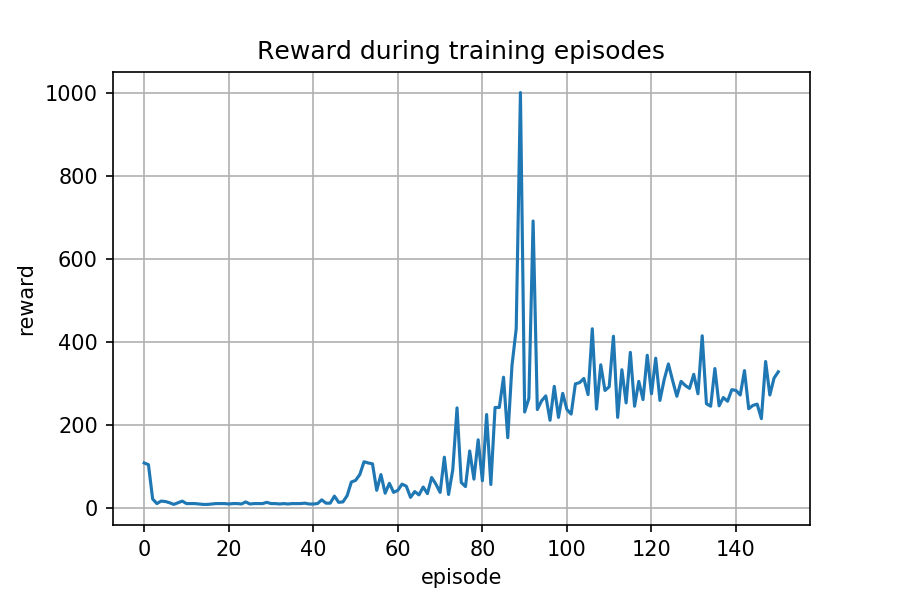
\includegraphics[width=11.70cm, height=7.9cm]{plots/cartpole_episode_reward.png}
	\caption{
		\label{fig:cartpole_episode_reward}
		TODO.
	}
\end{figure}

\begin{figure}[H]
	\centering 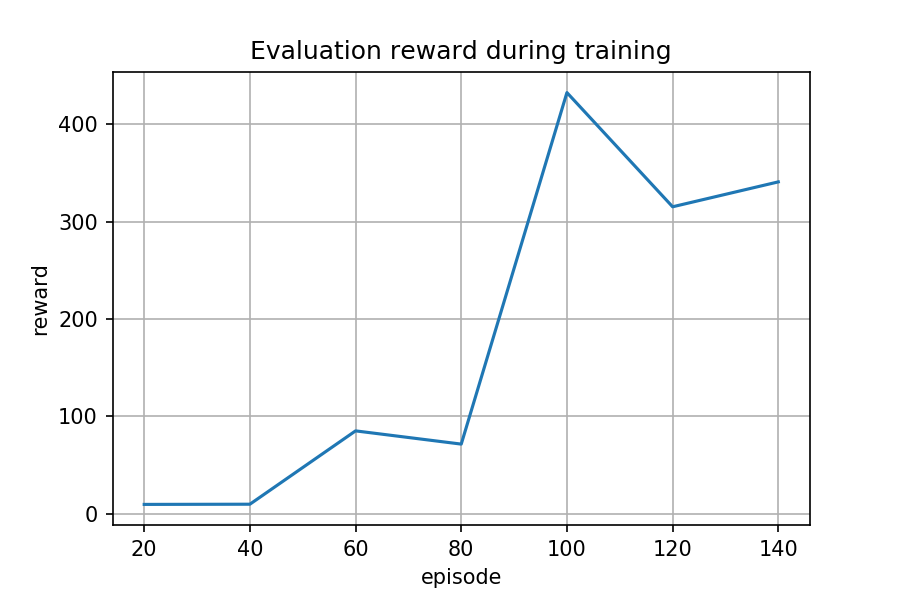
\includegraphics[width=11.70cm, height=7.9cm]{plots/cartpole_evaluation_reward.png}
	\caption{
		\label{fig:cartpole_evaluation_reward}
		TODO.
	}
\end{figure}

\subsection{CarRacing}\label{carracing}

%\begin{figure}[H]
%	\centering 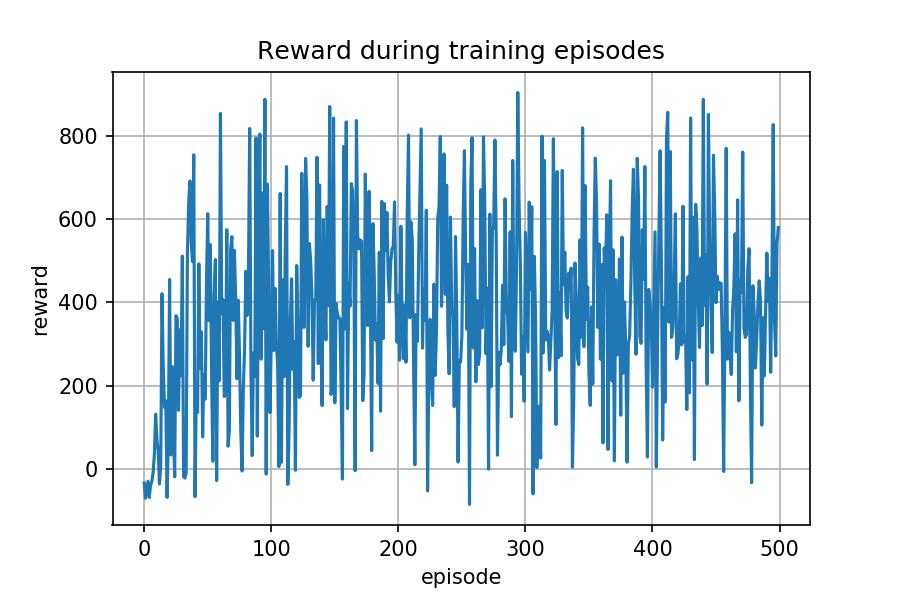
\includegraphics[width=11.70cm, height=7.9cm]{plots/carracing_episode_reward.png}
%	\caption{
%		\label{fig:carracing_episode_reward}
%		TODO.
%	}
%\end{figure}

%\begin{figure}[H]
%	\centering 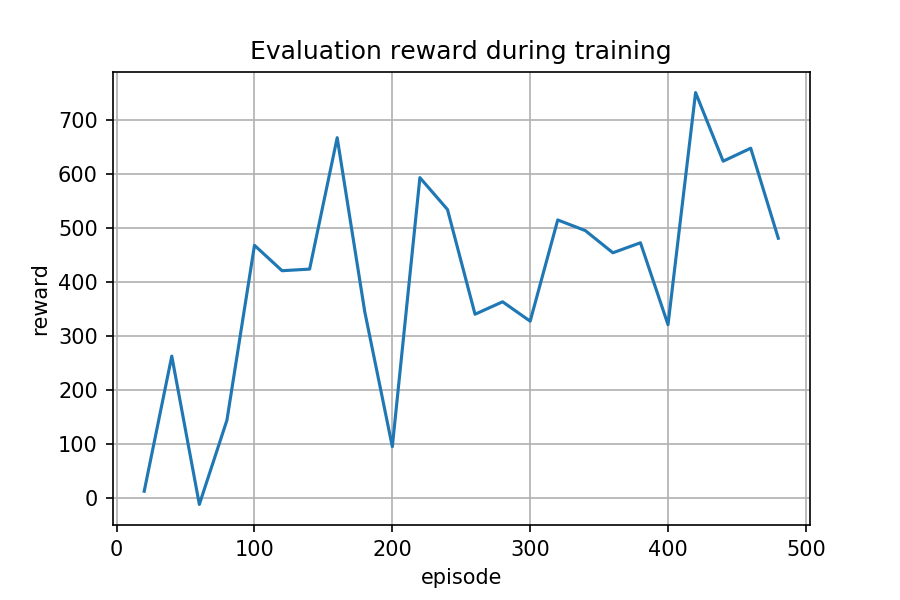
\includegraphics[width=11.70cm, height=7.9cm]{plots/carracing_evaluation_reward.png}
%	\caption{
%		\label{fig:carracing_evaluation_reward}
%		TODO.
%	}
%\end{figure}

\section{Conclusion}



\end{document}
